\documentclass[a4paper,12pt]{article} % тип документа
\usepackage[margin=1in]{geometry} % Поля

%  Русский язык
\usepackage[warn]{mathtext}
\usepackage[T2A]{fontenc}			% кодировка
\usepackage[utf8]{inputenc}			% кодировка исходного текста
\usepackage[english,russian]{babel}	% локализация и переносы
% Математика
\usepackage{amsmath,amsfonts,amssymb,amsthm,mathtools} 
\usepackage{wasysym}
%%%
\usepackage{graphicx}

\usepackage{tabularx}

\usepackage{gensymb} % знак градуса
\usepackage{enumitem} % изменить список enumerate
\usepackage{placeins} % \FloatBarrier

\renewcommand{\thesection}{\Roman{section}} 
\renewcommand{\thesubsection}{\roman{subsection}}


\begin{document}

\newcolumntype{Y}{>{\centering\arraybackslash}X} %new tabularx


%титул
\hrule 	
\medskip
\begin{raggedright}
{\large \textbf{Отчёт по работе 6.9.1}}
\\
\medskip
{\Large Закон Кюрий-Вейсса и обменное взаимодействие в ферромагнетиках} 
\\
\medskip
{\large Карташов Константин Б04-005}
\medskip
\hrule
\medskip
\end{raggedright}


\paragraph{Цель работы:} 
	Исследуется температурная зависимость магнитной восприимчивости ферромагнетика в парамагнитной области -- выше точки Кюри. По полученной в работе температуре Кюри оценивается энергия обменного взаимодействия. Объектом исследования является металлический гадолиний.

\medskip\hrule\medskip

\section{Теоретическая часть}

\paragraph{}
	Намагниченность вещества $I$ связана с внешним магнитным полем $H$, под воздействием которого она возникает, соотношением 
	\[
	I = \varkappa H,
	\]
	где $\varkappa$ называется магнитной восприимчивостью. Для парамагнитного вещества, в котором магнитный момент атома обусловлен спином одного электрона:

	\[
	\varkappa = \dfrac{I}{H} = N\dfrac{\mu^2}{k_{\text{Б}}T}.
	\]
	
	Для атома с более чем одним электроном и суммарным спином $S$, эта формула обобщается как
	\begin{equation}
	\varkappa = \dfrac{Ng^2 \mu_{\text{Б}}^2S(S+1)}{3k_{\text{Б}}T}
	\label{e:paramag}
	\end{equation}
	где $g$ -- фактор Ланде.

\paragraph{}
	В ферромагнетиках для описание взаимодействия соседних электронов вводится эффективное (или обменное) поле $H_{\text{эфф}}$, величина которого пропорциональна намагниченности:
	\[
	H_{\text{эфф}} = \lambda I,
	\]
	где $\lambda$ -- некоторая константа. С учётом этого поля формула \eqref{e:paramag} примет вид:
	\[
	\varkappa = \dfrac{I}{H} = N\dfrac{g^2 \mu_{\text{Б}}^2 S(S+1)}{3k_{\text{Б}}(T-\Theta)},
	\]
	где 
	\[
	\Theta = N \dfrac{g^2 \mu_{\text{Б}}^2 S(S+1)}{3k_{\text{Б}}}\lambda.
	\]
	
	В итоге получили соотношение:
	\begin{equation}
	\varkappa \propto \dfrac{1}{T - \Theta},
	\end{equation}
	называемое \textit{законом Кюри--Вейса}. Температура $\Theta$ называется парамагнитной точкой Кюри, при стремлении температуры к ней восприимчивость неограниченно возрастает из-за того, что тепловое движение всё меньше препятствует магнитным моментам ориентироваться в одном направлении.
	
\paragraph{}
	При учёте того, что энергия обменного взаимодействия умноженная на два это энергией изменения направления спина атома в поле $H_{\text{эфф}}$. Получим соотношение:
\[
\lambda = \dfrac{2nJV}{g^2\mu^2_\text{Б}}.
\]
 где $J$ -- обменный интеграл, $V = 1/N$ -- объём приходящийся на один атом. Из этого соотношения получим формулу для определения величины обменного интеграла:
\begin{equation}
J = \frac{3 k_\text{Б} \Theta}{2nS(S + 1)}.
\label{e:integral}
\end{equation}

\medskip\hrule\medskip

\section{Экспериментальная часть}

\subsection{Экспериментальная установка}

\paragraph{}
	На рис. \ref{fig:setup} показана схема экспериментальной установки для измерения восприимчивости магнетиков. Ферромагнитный образец 1 располагается внутри пустотелой катушки 2, которая является индуктивностью колебательного контура, входящего в состав LC-генератора. Частота колебаний генератора высвечивается на цифровом табло на блоке генератора. Катушка самоиндукции помещена в термостат 3. Для того чтобы в образце не возникали токи Фуко, маскирующие изучаемый эффект, он изготовлен из мелких гранул размером менее 0.1 мм. Образец помещен в тефлоновою капсулу. С помощью штока 5 капсулу можно перемещать вдоль оси катушки самоиндукции.

\begin{figure}[h]
\centering
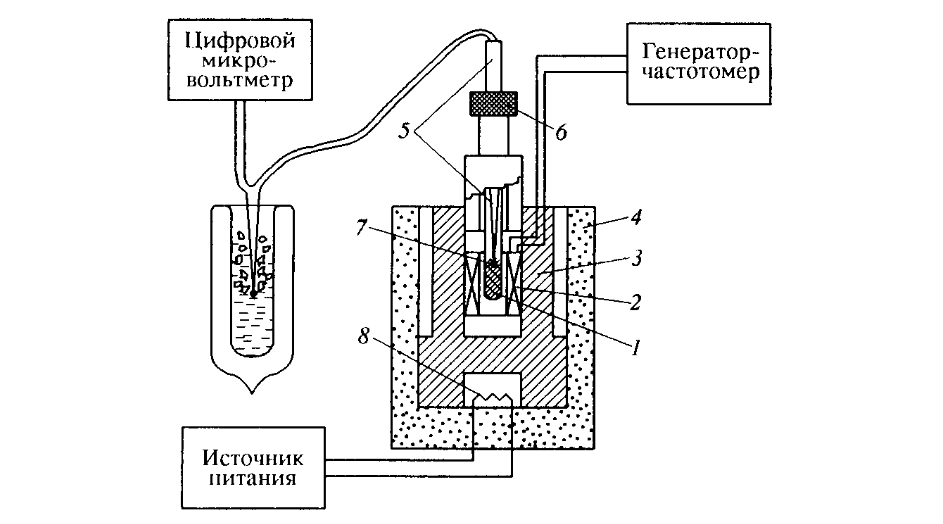
\includegraphics[width=0.7\textwidth]{setup.png}
\caption{Схема экспериментальной установки}
\label{fig:setup}
\end{figure}

\paragraph{}
	Магнитная восприимчивость определяется по изменению самоиндукции, происходящему при его введению в катушку. Обозначая через $L$ самоиндукцию катушки с образцом и через $L_0$ -- её самоиндукцию в отсутствие образца, получим:

\begin{equation}
L = \mu \frac{4 \pi n^2 S}{l}, \; L_0 = \frac{4 \pi n^2 S}{l},
\end{equation}

\noindent где $\mu$ -- магнитная проницаемость образца, $n$ --  число витков катушки, $l$ -- длина катушки, $S$ -- её сечение. Тогда, пренебрегая размагничивающим фактором, так как длина образца существенно больше его диаметра, получим:

\begin{equation}
\frac{L - L_0}{L_0} = \frac{\Delta L}{L_0} = \mu - 1 = 4 \pi \varkappa.
\end{equation}

\noindent Учитывая, что частота $f$ колебательного LC-контура определяется  выражением $1/f = 2 \pi \sqrt{LC}$, получим:

\begin{equation}
\frac{f_0^2 - f^2}{f^2} = 4 \pi \varkappa.
\end{equation}

\noindent Откуда следует, что:

\begin{equation}
\frac{1}{\varkappa} \propto \frac{f^2}{f_0^2 - f^2}.
\end{equation}

\paragraph{} 
	Температура образца измеряется медно-константановой термопарой, соединённой с цифровым вольтметром, с чувствительностью $\alpha^{-1} = 41$ мкВ/К. Измерения проводятся в интервале температур от 10\degree С до 70\degree С.

\subsection{Проведение измерений}

\paragraph{} 
	Убедившись в исправности установки приступим к охлаждению образца. После достижения образцом минимальной температуры начнём измерять значения $f_0$, $f$ и $U_\text{терм}$. Второй конец термопары находится при комнатной температуре $T_0 = 24$\degree C, в нулевом положении значение вольтметра $U_0 = 0.06$ мВ. 
	
	Температуру образца определим по формуле:
	
\begin{equation}
T = T_0 + \alpha \left(U_\text{терм} - U_0 \right),
\label{e:temp}
\end{equation}

\noindent погрешность определения температуры определяется ценой деления вольтметра $\Delta U = 0.01$ В, поэтому $\Delta T = \alpha \Delta U \approx 0.3$ К.

	Оценим погрешность рассчитываемой величины $f^2 / (f_0^2 - f^2)$ пользуясь стандартным подходом для оценки погрешности из чего получим:
	
\begin{equation}																				
\Delta \left( \frac{f^2}{f_0^2 - f^2} \right) = \frac{2 f^2}{f_0^2 - f^2} \sqrt{\left( \frac{\Delta f}{f} \right)^2 + \left( \frac{\sqrt{(f_0 \Delta f_0)^2 + (f \Delta f)^2}}{f_0^2 - f^2} \right)^2},
\label{e:fvalue_eror}																																																					
\end{equation}											

\noindent видим, что погрешность будет высокой при $f_0 \approx f$, погрешность измерения частоты $\Delta f = \Delta f_0 \sim 0.5$ кГц возникает в основном за счёт быстрого изменения показаний частотомера (за время необходимое для измерения $f$ и $f_0$ показания этих величин меняются на $\Delta f$), что вероятно связанно с постоянным изменением температуры. Измеренные и рассчитанные данные приведены в таблице \ref{tab:data} (величина $f^2 / (f_0^2 - f^2)$ обозначена как $y$).

\begin{table}[]
\centering
\begin{tabular}{|l|l|l|l|l|l|}
\hline
$U_\text{терм}$, мВ & $f$, кГц & $f_0$, кГц & $T$   & $y$  & $\Delta y$ \\ \hline
-0.66               & 809.9    & 867.4      & 279.4 & 6.80 & 0.08       \\ \hline
-0.59               & 810.1    & 867.3      & 281.1 & 6.84 & 0.09       \\ \hline
-0.5                & 810.3    & 867.3      & 283.3 & 6.87 & 0.09       \\ \hline
-0.39               & 810.7    & 867.5      & 286.0 & 6.89 & 0.09       \\ \hline
-0.29               & 812.6    & 867.6      & 288.5 & 7.15 & 0.09       \\ \hline
-0.18               & 820.4    & 867.4      & 291.1 & 8.5  & 0.1        \\ \hline
-0.08               & 837.1    & 867.8      & 293.6 & 13.4 & 0.3        \\ \hline
0.02                & 850.1    & 868.3      & 296.0 & 23.1 & 0.9        \\ \hline
0.12                & 858.5    & 868.3      & 298.5 & 44   & 3          \\ \hline
0.22                & 862      & 868.7      & 300.9 & 64   & 7          \\ \hline
0.32                & 864      & 868.3      & 303.3 & 100  & 16         \\ \hline
0.42                & 864.8    & 868.7      & 305.8 & 111  & 20         \\ \hline
0.53                & 865.8    & 868.5      & 308.5 & 160  & 42         \\ \hline
0.63                & 866.3    & 869.2      & 310.9 & 149  & 36         \\ \hline
0.72                & 885.9    & 887.2      & 313.1 & 340  & 185        \\ \hline
0.8                 & 888.6    & 891.2      & 315.0 & 171  & 46         \\ \hline
0.84                & 891.5    & 893.8      & 316.0 & 194  & 60         \\ \hline
0.86                & 892.9    & 895        & 316.5 & 212  & 72         \\ \hline
\end{tabular}
\caption{Измеренные и рассчитанные данные.}
\label{tab:data}
\end{table}

\subsection{Определение температуры Кюри и величины обменного интеграла}

\paragraph{}
	Построим график зависимости $[f^2 / (f_0^2 - f^2)](T)$ по данным из таблицы \ref{tab:data} (рис. \ref{fig:plot}). По графику определим участок, на котором зависимость будет линейной, по точкам из этого участка построим линейную аппроксимацию (y = ax + b) методом наименьших квадратов с весом точек равным обратной погрешности $w = 1 / \Delta y$. Полученные коэффициенты $a = 8.8 \pm 0.3$, $b = -2570 \pm 90$ К. 
	
	Определим температуру Кюри из условия $y = 0$, из чего получаем:
	
\[
\Theta = - \frac{b}{a} = \frac{2570 \text{ К}}{8.8} = 292 \text{ К},\]
\[
\Delta \Theta = \Theta \sqrt{\left( \frac{\Delta a}{a} \right)^2 + \left( \frac{\Delta b}{b} \right)^2} = 292 \sqrt{\left( \frac{0.3}{8.8} \right)^2 + \left( \frac{90}{2570} \right)^2} = 14 \text{ К},
\] 

\noindent то есть из измерений $\Theta = 290 \pm 15$ К.

\paragraph{}
	По формуле \eqref{e:integral} определим величину обменного интеграла, полагая $n = 12 , S = 7/2$:
	
\[
J = \frac{3 k_\text{Б}}{2nS(S + 1)} \Theta = \frac{3 \cdot 1.38 \cdot 10^{-16} \text{ эрг/К}}{2 \cdot 12 \cdot 3.5 \cdot 4.5} \cdot 290 \text{ К} = 3.18 \cdot 10^{-16} \text{ эрг} = 198 \text{ мкэВ},
\]\[
\Delta J = J \frac{\Delta \Theta}{\Theta} = 198 \cdot \frac{15}{290} = 10 \text{ мкэВ},
\]

\noindent получили $J = 200 \pm 10$ мкэВ $ = 7.9 \pm 0.4$ К.


	
	
\begin{figure}[h]
\centering
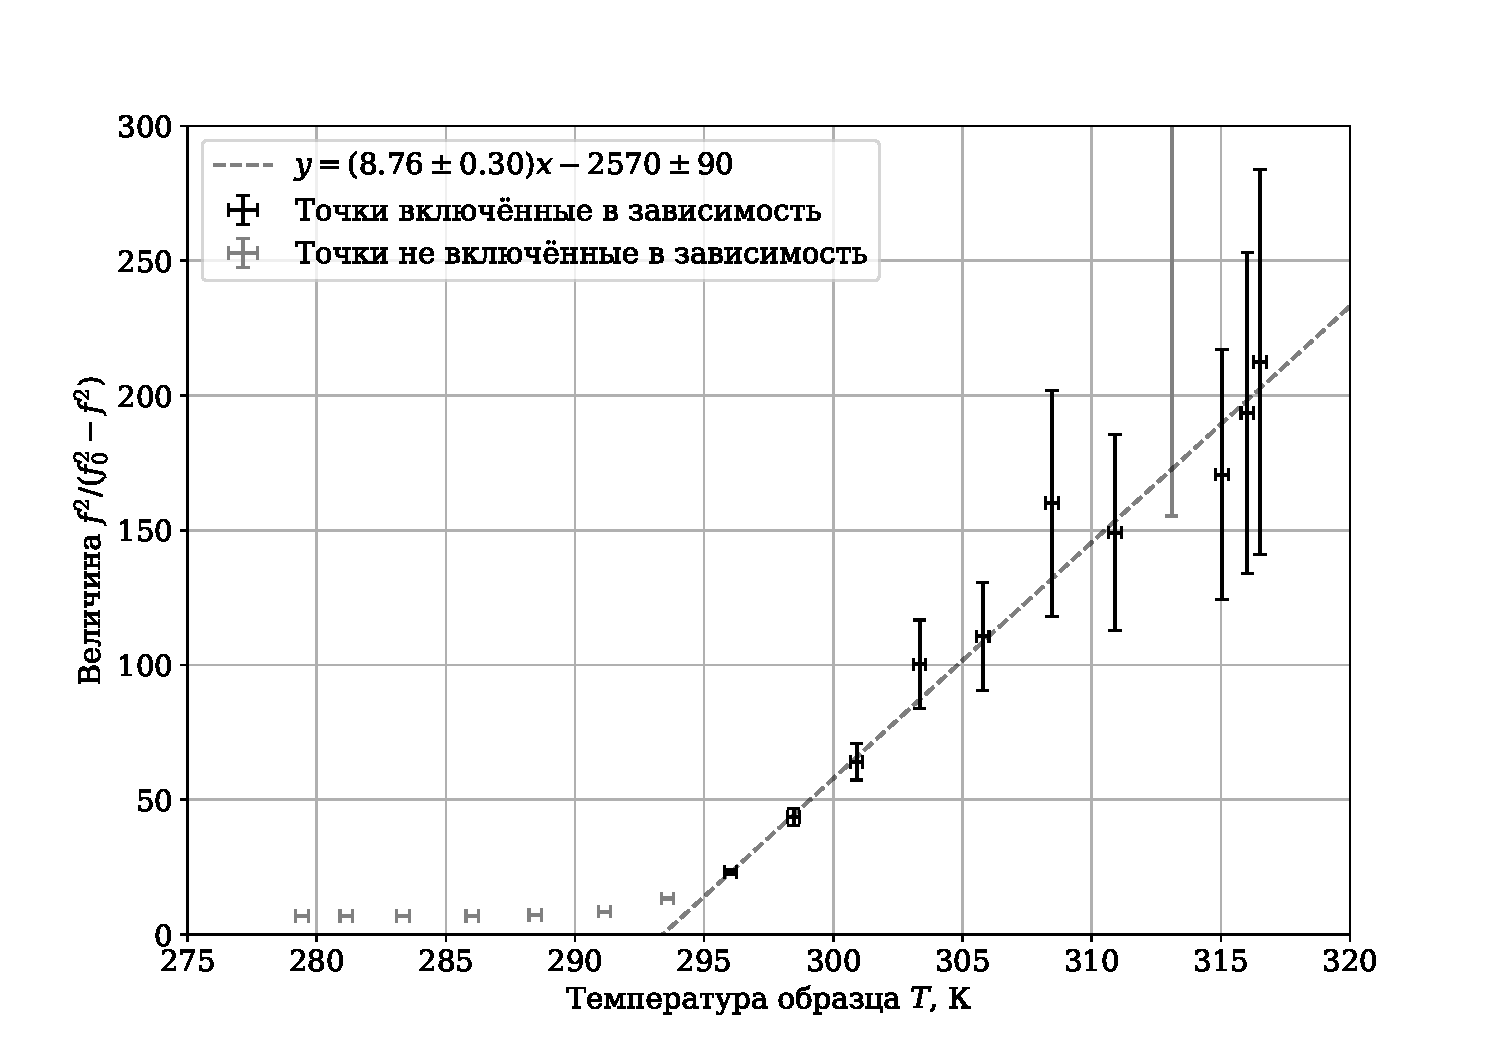
\includegraphics[width=\textwidth]{plot.pdf}
\caption{График зависимости $[f^2 / (f_0^2 - f^2)](T)$ с аппроксимацией линейного участка}
\label{fig:plot}
\end{figure}


\medskip\hrule\medskip

\section{Выводы}

\begin{enumerate}
\item Изучили температурную зависимость магнитной восприимчивости гадолиния. Показали, что при переходе через точку Кюри эта зависимость резко изменяется.
\item По полученной температурной зависимости нашли точку Кюри. $\Theta = 292 \pm 14$ К. Что хорошо согласуется с табличным значением $\Theta = 292$ К.
\item По полученной точке Кюри вычислили величину обменного интеграла $J = = 200 \pm 10$ мкэВ $ = 7.9 \pm 0.4$ К.
\end{enumerate}



\medskip\hrule\medskip

\end{document}
